\subsection{Deep Learning Tasks}
The following deep learning tasks are related to our objectives.
\begin{enumerate}
    \item \textbf{Semantic segmentation}\newline
\textcolor{gray}{In order to get the drivable region, one of the important steps is to do semantic segmentation.  The most influential work in the field of semantic segmentation up to authors' best knowledge is \textit{Deeplabv3+} by Google. By employing an encoder-decoder structure, the encoder module encodes multi-scale contextual information by
applying atrous convolution at multiple scales. Deeplab demonstrates the effectiveness of the proposed model on \textit{PASCAL VOC 2012} and \textit{Cityscapes datasets}, which respectivelly attain the test set performance of 89.0\% and 82.1\% without any post-processing. \cite{Chen2018DeepLab}}

\item \textbf{Object Detection}\newline
\textcolor{gray}{Another important part in our project is object detection, which is aimed to classify pedestrians, cars, buses etc. There are several neural network architectures available, and YOLO (You Only Look Once) \cite{Redmon2018YOLOv3} is a state-of-the-art, real-time object detection system. 
The model has several advantages over classifier-based systems. It looks at the whole image at test time so its predictions are informed by the global context in an image. Unlike systems such as R-CNN requiring thousands of network evaluation for a single image, it makes predictions with a single one. Such advantage makes it extremely fast, more than 1000x faster than R-CNN and 100x faster than Fast R-CNN. Also, it produces good results: it has a mean average precision (mAP) of 57.9\% on COCO test-dev. }

\item \textbf{Human Pose Detection}\newline
\textcolor{gray}{In order to get the future trajectory of a pedestrian, it is important to know his/her pose and places of joints. Some work use a person detector and perform single-person pose estimation for each detection. Such top-down approaches have drawbacks: the more the people, the greater the computational cost. The
seminal work of Zhe Cao et al. \cite{Cao2016Realtime} used Pars Affinity Field (PAF), jointly learning parts detection and parts association. We will extend this work to have some intermediate layer information in order to help with the labeling. }
\end{enumerate}

\begin{figure}[h!]
  \centering 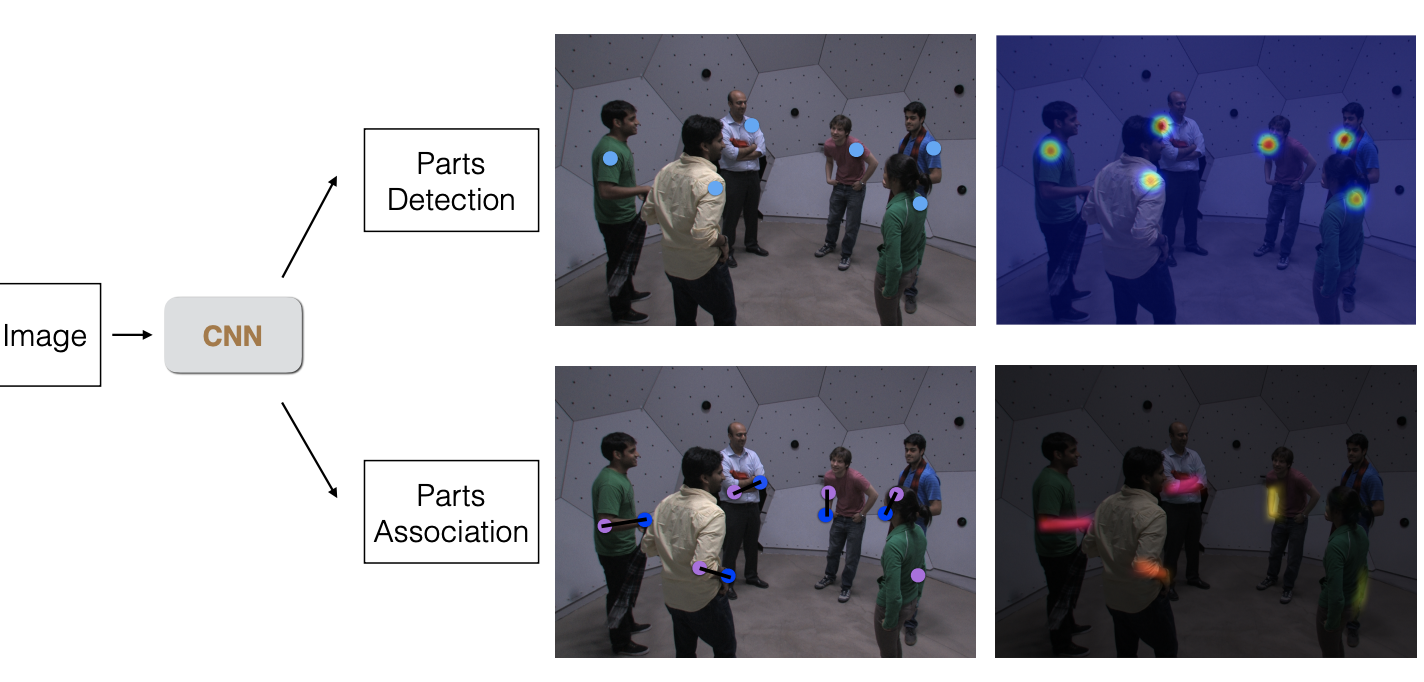
\includegraphics[width=\linewidth]{PAF.png}
  \caption{PAF Model Sample Output}
  \label{fig:PAF}
\end{figure}
